\normaltrue
\correctionfalse

%\UPSTIidClasse{11} % 11 sup, 12 spé
%\newcommand{\UPSTIidClasse}{12}

\exer{Mouvement RR  $\star$ \label{B2:13:PTSI:04:02}}
\setcounter{numques}{0}
\UPSTIcompetence{B2-13}
\index{Compétence B2-13-PTSI}
\index{Mécanisme à 2 rotations}
\ifcorrection
\else
\textbf{Pas de corrigé pour cet exercice.}
\fi

\ifprof
\else
Soit le mécanisme suivant. 
\begin{center}
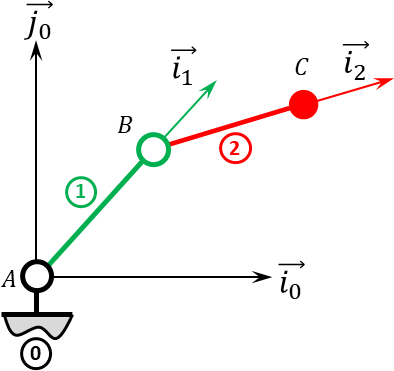
\includegraphics[width=\linewidth]{04_RR_01}
\end{center}
\fi

\question{Réaliser le paramétrage du mécanisme.}
\ifprof ~\\
\else

\fi



\ifprof
\else
\footnotesize

\normalsize
\begin{flushright}
\footnotesize{Corrigé  voir \ref{B2:13:PTSI:04:02}.}
\end{flushright}%
\fi